\documentclass[letterpaper]{article}
\usepackage[utf8]{inputenc}
\usepackage{authblk}
\usepackage{hyperref}
\usepackage{graphicx}
\usepackage[usenames,dvipsnames,svgnames,table]{xcolor}

\definecolor{teal}{HTML}{008080}

\hypersetup {
  colorlinks = true, linkcolor = teal, citecolor = teal, urlcolor = teal,
  pdfauthor = {Beauchesne, David},
}

\renewcommand\Affilfont{\itshape\small}
\setcounter{section}{-1}

\begin{document}

\title{
  \uppercase {Thinking outside the box - predicting biotic interactions in data-poor environments}
}
\uppercase{

\author[1*]{\textit{David Beauchesne}}
\author[2]{\textit{Philippe Desjardins-Proulx}}
\author[1]{\textit{Philippe Archambault}}
\author[2]{\textit{Dominique Gravel}}
}
\affil[*]{email: \href{mailto:david.beauchesne@uqar.ca}{david.beauchesne@uqar.ca}}
\affil[1]{Universit\'e du Qu\'ebec à Rimouski}
\affil[2]{Universit\'e de Sherbrooke}
\date{\today}
\maketitle

%ADD RUNNING TITLE HERE, MUST NOT EXCEEN 55 CHARACTERS AND SPACES

%UP TO 8 KEYWORDS
% \keywords{predicting biotic interactions, machine learning, food webs, estuary and gulf of St.Lawrence}



%------------------------------------------------------------------------------------------------------------------------
% Notes:
% Valoriser la compilation des données et la méthodologie utilisée pour atteindre les objectifs. Article d'avantage méthodologique.
%
% Objectif: décrire les interactions pour une communauté pour laquelle peu d'interactions sont connues, ou indisponibles.
%

\newpage
\section{Timeline}
  \begin{table}[h!]
    \centering
    \begin{tabular}{l c}
      \hline
      Work accomplished                                           & Approx. time   \\
                                                                  & (months)    \\
      \hline
      Discussions and research for data compilation               & 0.5         \\
      Empirical webs formatting                                   & 2           \\
      GloBI extractions                                           & 0.5         \\
      Taxonomy                                                    & 0.5         \\
      Data catalogue compilation                                  & 0.75        \\
      Two-way Tanimoto algorithm first iteration                  & 0.25        \\
      \hline \hline
      \textit{Total}                                              & \textit{4.5}  \\
      \hline
      \\
      \hline
      Work to do in perfect world                                 & Predicted time    \\
                                                                  & (days)      \\
      \hline
      \textbf{\textit{Analyses and associated code}}                            \\
      Analysis plan                                               & 0.5         \\
      Finalize two-way Tanimoto algorithm (w\/o similarity graph) & 1-2         \\
      Coding for analyses and figures                             & 3-4         \\
      Run analyses                                                & 2-4         \\
      \\
      \textbf{\textit{Writing}}                                                 \\
      Readings                                                    & 2           \\
      Introduction                                                & 2           \\
      Methods (machine learning, analyses)                        & 0.5         \\
      Results                                                     & 1           \\
      Discussion                                                  & 3           \\
      Appendix (list of food webs and references for catalogue)   & 0.5         \\
      Formatting                                                  & 1           \\
      \hline \hline
      \textit{Total}                                              &\textit{16.5 - 20.5} \\
      \hline
    \end{tabular}

    \caption{List of tasks accomplished and approximate timeline for tasks remaining. The predicted times for tasks left assume that nothing goes wrong (something always does) and that I will not need to exchange any further with Phil on the analyses (which will likely happen). It also assumes work full-time, which will not be the case in august. I will be in Sept-Îles from July 26\textsuperscript{th} to August 6\textsuperscript{th}, and then on the Teleost from August 16\textsuperscript{th} to September 2\textsuperscript{nd}, during which time I will not be able to work full-time on these tasks.}

    % \label{table:tanimoto}
  \end{table}

\newpage
\section{Contingency plan}
The total predicted time for the tasks remaining is 16.5 to 20.5 days if everything goes according to plan, working full time and assuming no more interactions are needed with Phil for the analyses. It is therefore likely that this work cannot be finished until September-October. A contingency plan must therefore be defined:
\\
\par\textbf{\textit{Methods perspective piece}} \\
\hangindent=0.7cm \textit{Solution}: Present methodology and test simple community of known organisms with algorithm as is as an example of it's use \\
\hangindent=0.7cm \textit{Pros}: less analyses, less writing \\
\hangindent=0.7cm Cons: burn methodology paper that could be published in better journal, especially if the results are interesting, which they very well might be. Except if we turn it in a way that allows us to publish two papers from the methodology presented. \\
\\
\par\textbf{\textit{No idea...}} \\
\hangindent=0.7cm \textit{Solution}:  \\
\hangindent=0.7cm \textit{Pros}:  \\
\hangindent=0.7cm \textit{Cons}:  \\
\\
\par\textbf{\textit{Abandon submission}} \\
\hangindent=0.7cm \textit{Solution}: \dots \\
\hangindent=0.7cm \textit{Pros}: less everything, take the time to finish the paper with a solid methodology and, if results are good, submit to a better and more targeted journal \\
\hangindent=0.7cm \textit{Cons}: lose a paper, not respect engagements (major con \dots) \\

\section{In the interim \dots}
\begin{enumerate}
  \item I am continuing to run analyses and generating similarity matrices for multiple parameter values, as the bottleneck for the analyses is there.
  \item I have a fully resolved version of the St. Lawrence food web, which cannot be validated.
  \item I am coding for the analyses to perform in the original scenario
  \item I am trying to write as much as possible in down times, which will be less often now that I have left for the field
  \item Putting together a very simple community matrix with known species to test the algorithm on and provide an easy working example (assuming it works). See more details in the next section.
\end{enumerate}

\section{Simple working example}
I need to choose a simple example to verify the Algorithm as it is currently coded. I could take the ecopath model of the southern gulf of st.lawrence and compare predictions with the diet matrix used in the EwE model. We might want to choose something else even more simple, but more accurate. I believe that the EwE model only includes large taxonomic groups, but I will have to double check.

Steps:
 \begin{enumerate}
   \item Load EwE model data (or other community)
   \item Format taxa nomenclature
   \item Extract taxonomy
   \item Run Algorithm
   \item Compare predicted vs observed
 \end{enumerate}



\newpage
\section{Abstract}
% about 200 words, much too long at this point

Ecological communities, whose structure is largely defined by how species interact, forms the biological backbone of ecosystems. Large networks are complex to characterize, be it empirically or theoretically. The former requires exhaustive observations, while the latter generally requires ample data to be validated. Although large empirical datasets describing consumer-resource interactions are increasingly available, the ecosystems described are still few and far between. We therefore wondered whether available data, albeit originating from \textit{a variety of} ecosystems, could be used to predict species interactions in data deficient ecosystems. A potential resolution for this issue lies in the taxonomic proximity between species, which increases their likelihood of sharing both consumers and resources. To test this, we built a biotic interaction catalogue from a collection of \textit{94} empirical food webs, detailed predator-prey interaction databases and interactions from the Global Biotic Interaction (GloBI) database. We used an \textit{unsupervised machine learning method} to predict the topology of the St. Lawrence food web, in eastern Canada, given the pairwise taxonomic proximity of St. Lawrence species with taxa found in the interaction catalogue. We find that food web topology can be predicted with high accuracy, which increases as the number of taxa in the network increases. The taxonomic resolution at which interactions are defined influences results, with optimal prediction accuracy at the genus level. Prediction accuracy also varied between large taxonomic groups, with fish and mammals attaining a much higher prediction accuracy than benthic invertebrates, reflecting the unequal distribution of data available between taxonomic groups.



Given it's high accuracy, this methodology could democratize the use of food webs and network level descriptors :
\begin{itemize}
\item in remote location where empirical data is hard to gather
\item impact assessments by curtailing the initial exhaustive empirical description of networks. Network characteristics could then be efficiently evaluated and correlated to levels of environmental stressors.
\end{itemize}

Methodology could also extended to quantitatively eveluate interaction strength between taxa % Dom's idea


\section{Introduction, last paragraph}

Thus, can we take advantage of available data to predict biotic interactions in data-poor environments? The objective of this paper is to use the link between taxonomic proximity and shared interactions to build models predicting biotic interactions in data poor ecosystems.

\section{Figures et tableaux}

\textit{Tables:}
\begin{enumerate}
  \item Description of empirical data used to obtain list of binary interactions
  \item Description of empirical binary interactions and data availability for large taxonomic groups (e.g. mammals, fish, benthic invertebrates). Needs to be defined.
\end{enumerate}

\textit{Figures:}
\begin{enumerate}
  \item Predicting empirical food webs from empirical data catalogue. Figure of results \% efficiency as a function of the number of taxa in the food web. All species-species interactions of each empirical food web removed from empirical biotic interaction catalogue.
  \item Predicting interactions with differing levels of taxonomic resolution. (e.g. interactions aggregated at the species, genus, family level)
  \item Efficiency of predictions for large taxonomic groups.
  \item Representing the St. Lawrence food web. Heatmap with phylogeny as axes. Package heatmap3.
\end{enumerate}

\textit{Figure additionnelle mais peut-être pas pour cet article?:}
\begin{enumerate}
  \item Predictive accuracy of method as a function of the amount of data available in the catalogue for large taxonomic groups. The idea would be to discuss the amount of data required in ``biological compartments'' for the learning method to be efficient.
\end{enumerate}


%----------------------------------------------------------------------------
%----------------------------------------------------------------------------
%----------------------------------------------------------------------------
\section{\uppercase {No need to read the rest}}


\section{Introduction}
% À venir

% Interactions are described for a limited amount of taxa in varying types of environments.
%
% Describing the structure of a community often requires a thorough understanding of species composition and interactions locally. This kind of knowledge is often lacking.
%
% Species that are taxonomically closely related are thought to have a higher probability of sharing similar types predators and preys (refs). Based on that assumption, taxonomy could be used as a proxy to predict biotic interactions between taxa.
%
% Identify species that are likely to interact in any given environment by training models with empirical data coming from other communities.
%
% based on their taxonomic or phylogenetic proximity
%
% Our objective was therefore to test whether we could predict species interactions in a given community using empirical data gathered from other communities.


% So the idea:


% 1st par.: Challenge of fully describing interactions in a community.

% Notes:
%   J'aime pas ce paragraphe, mais il donne quand même une bonne idée de ce que je veux avancer comme premier paragraphe, surtout la première et la dernière phrase. Du moins jusqu'à ce que je détruise ce que j'ai écrit pour le reformater...

To include in introduction: interactions can also be predicted by functional traits such as body size and metabolism type (e.g. Gravel et al 2013;), yet even those can be difficult to extensively characterize for multiple taxa. We therefore sought more readily available information for all taxa of interest.

We therefore turned our attention towards phylogenies, taxonomies, to get more readily available data for each taxon of interest


The study of ecosystem structure and function is increasingly focusing on communities of interacting species that form the biological backbone of ecosystems. Fully describing consumer-resource interactions can however be a daunting task due tho the sheer number of potential interactions, even for a limited number of species (Dodds and Nelson 2006). The empirical description of interactions at the community scale can thus be limited by logistical constraints (Dunne 2006; Morales-Castilla et al. 2015). In the context of environmental impact evaluation, the time required to gather empirical data can further diminish the applicability of such methodologies due to time constraints (ref).

% -----------------------------
% 2nd par.: Predicting interactions based on traits and phylogenies (See, among others, Eklof)

% Notes:
%   Find other references for first sentence, it's looks like auto-citation a lot: (e.g. Gravel et al., 2013; Albouy et al., 2014; Morales-Castilla et al., 2015).

  % 'Because of shared evolutionary history, closely related species typically have similar traits [13], which in turn determine their trophic interactions. As such, similar species are more likely to consume or be consumed by similar species [8,14,15]. Evolutionary history could possibly then be used as a surrogate for trophically important traits. Therefore, it is likely that we could detect a signature of evolutionary history in the structure of food webs where closely related species should have specific patterns of interactions (Eklof et al. 2012, citation).' ?
  % They explain it better than I do and I assume that my paragraph is much less interesting, to the point, relevant and factually correct. Plus, the second has absolutely no references to back it up, as everything essentially comes from Eklof et al 2012.

  % 'Consumers are organized in groups forming a nested hierarchy, which better reflects the complexity and multidimensionality of most natural systems' Cattin et al. 2004

Alternative approaches to predicting interactions among community members have thus been explored in order to efficiently resolve interaction webs using incomplete, imperfect or even unavailable data (e.g. Gravel et al., 2013; Morales-Castilla et al., 2015). These approaches rely on the use of proxies such as functional traits to infer interactions consumer-resource relationships (Morales-Castilla et al. 2015). Multiple traits can play a significant role in community dynamics and influence the presence and intensity of biotic interactions, like the influence of body size on predator-prey interactions, a literal take on \textit{big fish eats small fish} (Cohen et al., 2003; Brose et al., 2006; Gravel et al. 2013).

Evolutionary processes causes closely related species to share similar traits. This proximity increases the likelihood of closely related species sharing consumer and resources. Furthermore, trait differentiation arises through evolution, dictated by the coevolutionary dynamics and trait matching of consumers and resources. It is therefore likely that phylogenies could serve as proxies of important traits and, by extention, help predict pairwise interactions.

% -----------------------------
% 3rd par.: Methodologies for interaction predictions: Machine-learning algorithms. Need large datasets to 'learn from'.



% -----------------------------
% 4th par.: Preexisting data available in different environment. Can we make use of the relationship between evolutionary processes and consumer-resource trait matching to construct large datasets from which we can infer other species interactions?
These methodologies require large datasets from which models must be trained. There exist a large collection of empirical data that could be used to train such models. However, this collection comes from a wide variety of species and ecosystems.

Could we make use of such data to predict interactions in a given community in which knowledge is lacking, based on the phylogenetic proximity of species. Is it a truism to say that a species spatially distant from each other are likely to consume other species that are closely related phylogenetically?


% -----------------------------
% 5th par.: Objective and predictions


  Can we make use of existing heterogeneous data to predict interactions in a given community % Find better term than heterogeneous for this. I want to say that the data comes from many different studies, areas and types of ecosystems

The goal is to obtain a fully or optimally resolved interaction matrix for all taxa in a given community, i.e. constructing the community metaweb, or its topology (Dunne 2006).



  Consumer-resource trait matching dictate the interactions in a given community
  Trait differentiation arise through evolution, dictated by the coevolutionary dynamics of consumer-resource




\section{Methods}
  \subsection{Gap-filling algorithm} %or whatever of the methods will be
  % À venir
  % Lire 15
  % Faire un diagramme décisionnel qui montre les étapes de l'algorithme?

  % NOTES:
  %   In this version of the algorithm, we use similarity matrices rather than graphs, which greatly slows down the analysis speed.
  %   We therefore divide the algorightm between :
  %     Similarity evaluation (functions: similarity_taxon & similarity_taxon_to_predict, 'wt' argument has to be the same for both functions)
  %     Interaction predictions (function: two_way_tanimoto_predict)
  %
  % Process steps for analyses:
  %   1. Similarity between taxa combinations
  %     1.1 Evaluate the similarity matrix of S0 (i.e. all species in catalogue) for a number of wt values seq(0, 1, by = 0.1)
  %     1.2 Define S1, set of species forming a community C[i] and for which we wish to predict interactions
  %     1.3 Remove all species in S1 from similarity matrix alreay measured and interactions stemming from C[i]
  %     1.4 Extend similarity matrix to include S1 taxa (Evaluate similarity for all additionnal combinations added to the matrix)
  %
  %   For each species in S1:
  %   2. Identify resources already known in interaction catalogue (S0) for S1 species
  %     2.1 If resoures are in S1, automatically add them to the predictions as empirically valid interactions
  %     2.2 If resources are not in S1, find Kr similar resources in S1 and add them to candidate list with weight equal to their similarity
  %
  %   3. Identify Kc similar consumers to S1 in S0
  %     3.1 Extract set of candidate resources from each similar consumer, if any
  %     3.2 If candidate resource is in S1, add it to candidate list with weight 1
  %     3.3 If candidate resource not in S1, find Kr similar resources in S1 and add them to candidate list with weight equal to their similarity
  %
  %   4. Make predictions:
  %     4.1 Remove taxa with weight < to minimum weight (MW) from prediction list
  %     4.2 Sort prediction list according to weight. Higher weights mean higher likelihood for resource being consumed
  %
  %   Subset of communities based on the number of taxa available? Most of them end up having very few taxa represented in here. Less than I expected...

Predicting interactions for a given community of taxa was performed using the \textit{K}-nearest neighbour (KNN) algorithm. This method predicts missing entries or proposes additional entries by a majority vote based on the \textit{K} nearest (\textit{i.e.} most similar) entries. In this case, species are described by a set of resources and their taxonomy.

The Tanimoto similarity measure compares two vectosr based on the number of elements they share and the number of elements they contain:

\begin{equation}
  tanimoto(\mathbf{x}, \mathbf{y}) = \frac{\sum_i x_i \land y_i}{\sum_i x_i \lor y_i},
\end{equation}

where $\land$ is bitwise \emph{and}, while $\lor$ is the bitwise \emph{or} operators.

This similarity measure can be expanded to consider sets of traits or a taxonomic description:

\begin{equation}
  tanimoto_t(\mathbf{x}, \mathbf{y}, w_t) = w_ttanimoto(\mathbf{x_t}, \mathbf{y_t}) + (1 - w_t)tanimoto(\mathbf{x_i}, \mathbf{y_i}),
\end{equation}

where $w_t$ is the weight given to traits or taxonomy, $\mathbf{x_t}$ and $\mathbf{y_t}$ are the vector of traits or taxonomy of two taxa, and $\mathbf{x_i}$, $\mathbf{y_i}$ are the resource vectors of the two taxa. When $w_t$ = 0 only resource vectors are used to compute similarity, while $w_t$ = 1 solely uses trait or taxonomy vectors.

% Still has to be done
We also evaluated a similarity measure exclusively applied to taxonomy, the XXX taxonomic similarity measure (ref):

\textit{Equation of taxonomic similarity}

\begin{equation}
  taxo(\mathbf{x}, \mathbf{y}, w_t) = w_ttaxo(\mathbf{x_t}, \mathbf{y_t}) + (1 - w_t)tanimoto(\mathbf{x_i}, \mathbf{y_i}),
\end{equation}





% Gap-filling algorithm,
% KNN machine learning method
% Tanimoto proximity measure
% Taxonomic proximity measure?
% Combining both proximity measure in the traits_tanimoto algorithm
%
% We extended the KNN algorithm with tanimoto similarity to include both consumer and resource similarity.
%
%
% Need to present the algorithm



  \subsection{Predicting interactions}
  % À mieux décrire et élaborer
We build the two-way Tanimoto algorithm in order to consider both the similarity between consumers and resources.

There is a minimum weight that is arbitrarily set by the user for candidate species to be included as predicted resources for a given taxa. The more often it comes up as a prediction, the more likely it will be included in the analysis. While this makes sense analytically, the number of resource per taxon in the interaction catalogue is not uniform (e.g. Atlantic cod has > 600 listed resources). Hence the more the candidate resources, the more likely a very small similarity value will give a predicted interaction. We had two choice to deal with this issue. Either we set a variable MW that varies as a function of the number of candidate resources, or we set another minimum threshold for resource to make it into the candidate list, effectively resulting in two arbitrarily chosen values for the predictions.

  \subsection{Data compilation}
  % Review in section:
    % Verify 'scientific nomenclature'
    % Number of empirical web used
    % Appendix 1 needed? Description of food web used. The majority come from GlobalWeb
    % GlobalWeb database (http://globalwebdb.com)
    % Verify references to add
    % GloBI; http://www.globalbioticinteractions.org
    % Verify number of taxa and number per taxa for first data compilation step


The empirical data used as prior knowledge to train our models and predict interactions between St. Lawrence species was compiled in two successive steps. The first consisted of gathering data from a collection of XXX empirical food webs in marine and coastal ecosystems (Brose et al. 2005; Kortsch et al. 2015; GlobalWeb database; see Appendix 1 for a description of food webs). We also used a detailed predator-prey interaction database describing trophic relationships between XX predators and their prey (Barnes et al. 2008). From these datasets, only interactions between taxa at the taxonomic scale of the family or higher were selected to go forward.

As empirical food webs are largely dominated by non-interactions, these datasets yielded a highly skewed distribution of interactions vs non-interactions. To counterbalance this, the second step of data compilation consisted of extracting observed interactions from the Global Biotic Interaction (GloBI) database (ref), which describes binary interactions for a wide range of taxa worldwide. We extracted all interactions available on GloBI for species belonging to the families of taxa identified in step 1 of data compilation and of St. Lawrence species. Interactions were extracted using the rGloBI package in R (ref). As for step 1, only interactions between taxa at the taxonomic scale of the family or higher were retained

The nomenclature used between datasets and food webs varied substantially. Taxa names thus had to be verified, modified to the scientific nomenclature and validated. This process was performed using the Taxize package in R (ref) and manually verified for errors. The same package was used to extract the taxonomy (\textit{i.e.} kingdom, phylum, class, order, family, genus, species) of all taxa for which interactions were obtained in previous steps.

We selected a list of species forming the known biodiversity of the estuary and gulf of St. Lawrence in Canada. The species list available on CaRMS (ref) for this region was selected, and completed with a comprehensive list of marine birds (Allard et al. 2013) and marine mammals (Lesage, personnal communication), for a total of 1469 species.

\subsection{Prediction accuracy}
% "We assessed the performance of our method using the True Skill Statistic (TSS). The TSS is based on the partition of events (the prediction of a trophic interaction) between four components: the component a reports the number of links that are both predicted and observed, b reports predicted links with no corresponding observation, c reports the number of observed links that are predicted absent and d reports the number of predicted and observed absence of links. The TSS is then calculated as TSS = (ad-bc)/[(a+c)(b+d)]. The TSS quantifies the proportion of prediction success relative to false predictions and returns values ranging between 1 (perfect predictions) and 1 (inverted forecast) (Allouche, Tsoar & Kadmon 2006)." Gravel et al. 2013 Body size




\section{Results}
% Notes:
% Figures à générer, suggestions:
%   1. Efficacité des prédictions
%   2. Efficacité des prédictions ~ quantité d'interactions empiriques
%   3. Efficacité prédiction ~ nombre de taxons
%   4. Efficacité ~ résolution taxonomique
%   5. Efficacité ~ grands groupes taxonomiques
%   6. Matrice d'interactions EGSL
%   7. Description des données extraites
%
% 1. Avec des réseaux complets ou simplement avec des taxons individuels?
%   - Pourrait sélectionner des réseaux bien décrits comme: Jacob ou Kortsch et al.
%   - Ensuite faire le Saint-Laurent
%   - Pourrait aussi simplement retirer un subset aléatoire des données itérativement pour les prédire (approche de Philippe dans son draft de manuscrit, 90-10)
%
% 2. Une proportion des taxons ont dû être extraits et ajustés manuellement pour des erreurs. Il s'agit de l'étape la plus chronophage, mais est-elle réellement nécessaire? De plus, c'est l'étape à laquelle le plus grand nombre d'erreurs peut se glisser à la base de donnée dû à l'erreur humaine. C'est aussi l'étape qui rend le travail plus difficilement reproductible puisque des choix externe sont fait par l'utilisateur. Est0ce qu'en sélectionnant unoquement les données valides dès le départ on obtient suffisamment de données pour obtenir des résultats satisfaisants?

% Ajouter une figure pour décrire les données disponibles pour les espèces, genre et famille du Saint-Laurent?

The data compilation process yielded a total of 276708 binary interactions (interactions = 72110; non-interactions = 204598) for 9712 taxa (Superfamily = 15; Family = 591; Subfamily = 29; Tribe = 8; Genus = 1972; Species = 7097). Of that number, interactions for St. Lawrence taxa were described for 33\% of species, 64\% of genera and 82\% of families, although these interactions are not necessarily between two taxa found in the St. Lawrence.


\subsection{First round of results}
So now we have the first round of results in. Here is how I interpret them in multiple points

We measure prediction accuracy based on four statistics:







 \begin{enumerate}
  \item \textit{TSS, the True Skilled Statistics quantifies the proportion of prediction success relative to false predictions and returns values ranging between 1 (perfect predictions) and 0 (inverted forecast) (Gravel et al. 2013)}
      \begin{equation}
        TSS = \frac{(ad - bc)}{(a + c)(b + d)}
      \end{equation}

  \item $Score_y$ is the fraction of interactions correctly predicted
      \begin{equation}
          Score_y = \frac{a}{a + c}
      \end{equation}

  \item $Score_{\neg y}$ is the fraction of non-interactions correctly predicted
      \begin{equation}
        Score_{\neg y}  = \frac{d}{b + d}
      \end{equation}

  \item Accuracy score is the normalized sum of correctly predicted interactions and interactions
  the sum(a, d) / sum(a, b, c, d)
      \begin{equation}
        Accuracy = \frac{a + d}{a + b + c + d},
      \end{equation}

 \end{enumerate}

 where a is the number of links predicted (1) and observed (1), b is the number predicted (1) but not observed (0), c is the number predicted absent (0) but observed (1) and d is the number of predicted absent (0) and observed absent (0).

 \begin{figure}
   \centering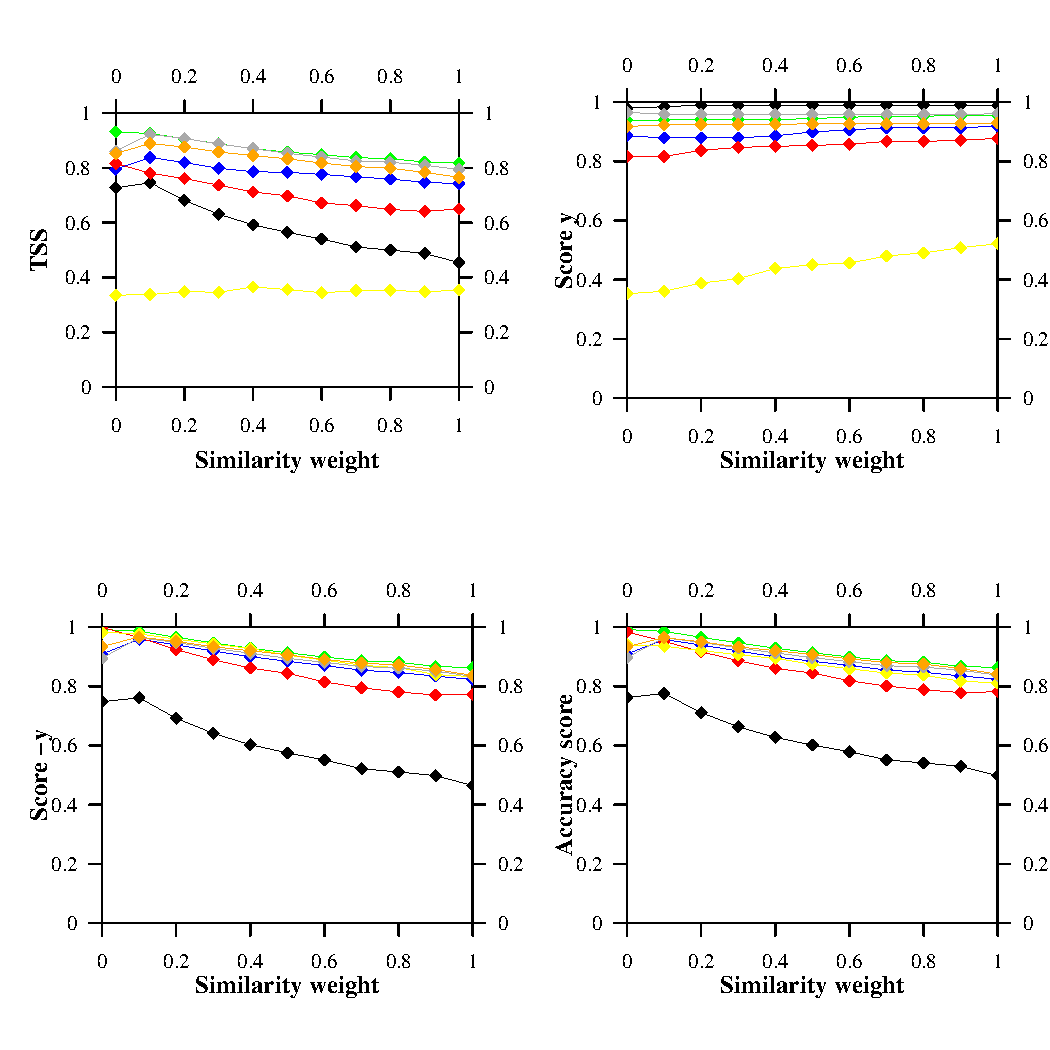
\includegraphics[width=0.85\textwidth]{results1.pdf}

   % \caption{}

   % \label{fig:}
 \end{figure}


The graph presents the four statistics as a function of trait weight, which varies between 0 and 1. A weight of 0 means that similarity is measured only using set of resources for each taxa, while a weight equal to 1 means that similarity is based solely on taxonomy. We present 6 food webs with over 50 taxa each and the Barnes et al. (2008) dataset.

The overall predictive power of the algorithm looks very interesting. Except for one food web, prediction accuracy varies mainly between 80\% to almost 100\% in certain cases. At first glance from the TSS and Accuracy score graphs, it may seem that the use of resource set only for similarity measurements (\textit{i.e.} wt = 0) yields better results than those with taxonomy (\textit{i.e.} wt = 1). However, caution must be exercised here. First, the catalogue was built from various sources that may have repeated values. While the catalogue itself only holds unique observations, it may very be the case that attempting to predict interactions of food webs from the catalogue with the catalogue may end up providing overinflated accuracy results, even if individual food web data are removed when predictions are made.

Secondly, there is the case of non-interactions. Looking at $Score_y$ and $Score_{\neg y}$, you can see that the trend in TSS and Accuracy score values are closely matching those of $Score_{\neg y}$. In opposition, the $Score_y$ are instead increasing with taxonomy being more important in the similarity measurements. There could be multiple explanations for this. First, the algorithm could simply perform poorly in predicting non-interactions, classifying them instead as interactions. However, I rather believe that the original empirical food webs are the ones doing poorly at observing non-interactions. Indeed, we assumed that non-interactions in empirical food webs meant that there were no interations between the species. However, most of the empirical webs had a strong focus attributed to higher order consumer species and very little attention given to other taxa (\textit{e.g.} benthic invertebrates). The catalogue of interactions, on the other hand, has a much broader focus than the original empirical webs. It therefore very well may be that wrongly classified non-interactions could indeed be real but unobserved interactions in natural systems.

This would need to be tested at some point, but right now the only thing we could do is measure the level of accuracy for different large taxonomic groups such as fish, mammals, birds, benthic invertebrates, zooplankton, etc.

This observation however raises the question of the utility of non-interactions in the analyses. At this point, the algorithm is coded to ignore non-interactions in the similarity measurements. Maybe it would make sense to do the same in the interpretation of the results itself. Or a third vector to the similarity measurements could be added that considers non-interactions as a set of resources not consumed by consumers (which we have in the data). Extended from this idea and the fact that taxonomically close species are more likely to share BOTH resources and predators, a fourth and fifth vector could also be added, corresponding to set of predators and set of non-predators, which we also have in the data. While set of predators would make sense as a third vector, more thought needs to be given to non-interactions stemming from empirical food webs and their actual value as observed data.

Another interesting thought from this is the potential use of GloBI on its own to perform automated and quick analyses. If non-interactions are deemed unecessary or of dubious quality, focusing only on observed interactions could lead to the creation of a platform on which interactions in a given system could be easily predicted from GloBI alone, or almost. GloBI interactions data already holds taxonomic classification. It's quality is however unfortunately not uniform and care must be taken when it is used. In any case, if only interactions are considered, then a third party platform could be built that uses the algorithm built in this paper, the GloBI data and a list of species for which we wish to predict the interactions.

In the meanwhile, there are multiple parameters that still need to be tested or adjusted in the algorithm, namely:
\begin{enumerate}
    \item taxonomic similarity measure instead of tanimoto similarity
    \item multiple K values for the algorithm (set at 5 for both consumer and resource in this case)
    \item multiple mean weight values, which determines the weight needed for candidate resources to be added to predicted resources in the algorithm
    \item in an ideal world, another completely independant food web that was not used in the catalogue. Alternatively, I could remove completely the species from the catalogue for similarity measurements, ultimately corresponding to giving all the similarity weight to taxonomy (wt = 1). It is therefore already done in this analysis by comparing wt = 1 to wt = 0.
    \item and multiple other analyses to verify the accuracy of the analyses (see list of tables and figures).
\end{enumerate}

\end{document}


% According to Eklof and Stouffer (2015), the phylogenetic component of food webs is a significant factor influencing the intervality of food webs. However, certain traits are not accounted by phylogenetic constraints, such as body size.

predict* specie* interaction*
